\documentclass[aspectratio=169,14pt,handout,notes]{beamer}
%\documentclass[aspectratio=169,14pt,handout,notes=only]{beamer}
%\documentclass[aspectratio=169,14pt,handout,notes=hide]{beamer}
\usepackage[utf8]{inputenc}
\usepackage{bbding}
\usepackage[weather]{ifsym}
\usepackage{color}
\usepackage{textgreek}
\usepackage{pgfpages}
\usepackage{transparent}
\usepackage{lmodern}    % just to avoid font size warnings



%\setbeameroption{hide notes} % Only slides
%\setbeameroption{show only notes} % Only notes
%\setbeameroption{show notes on second screen=right} % Both

% To give a presentation with the Skim reader (http://skim-app.sourceforge.net) on OSX so
% that you see the notes on your laptop and the slides on the projector, do the following:
%
% 1. Generate just the presentation (hide notes) and save to slides.pdf
% 2. Generate onlt the notes (show only nodes) and save to notes.pdf
% 3. With Skim open both slides.pdf and notes.pdf
% 4. Click on slides.pdf to bring it to front.
% 5. In Skim, under "View -> Presentation Option -> Synhcronized Noted Document"
%    select notes.pdf.
% 6. Now as you move around in slides.pdf the notes.pdf file will follow you.
% 7. Arrange windows so that notes.pdf is in full screen mode on your laptop
%    and slides.pdf is in presentation mode on the projector.

% Give a slight yellow tint to the notes page
\makeatletter
\defbeamertemplate{note page}{plain2}
{
  \pagecolor{yellow!5}
  \nointerlineskip
  \begin{minipage}{1.25\textwidth} % this is an addition
  \insertnote
  \end{minipage}               % this is an addition
}
\setbeamertemplate{note page}[plain2]

\setbeamertemplate{frametitle}
{
  \ifbeamercolorempty[bg]{frametitle}{}{\nointerlineskip}%
  \@tempdima=\textwidth%
  \advance\@tempdima by\beamer@leftmargin%
  \advance\@tempdima by\beamer@rightmargin%
  \pgfsetfillopacity{.7}       %<------ fix filling opacity
  \begin{beamercolorbox}[sep=0.3cm,left,wd=\the\@tempdima]{frametitle}
    \usebeamerfont{frametitle}%
    \vbox{}\vskip-1ex%
    \if@tempswa\else\csname beamer@fteleft\endcsname\fi%
    \strut\pgfsetfillopacity{1}\insertframetitle\strut\par%  <---- text opacity
    {%
      \ifx\insertframesubtitle\@empty%
      \else%
      {\usebeamerfont{framesubtitle}\usebeamercolor[fg]{framesubtitle}\insertframesubtitle\strut\par}%
      \fi
    }%
    \vskip-1ex%
    \if@tempswa\else\vskip-.3cm\fi% set inside beamercolorbox... evil here...

  \end{beamercolorbox}
}
\makeatother

\usepackage{graphicx}

\title{BizDevOps@Helsana}
\subtitle{Result based approach}
\author{Bastian Bukatz}
\institute{Innovation Process Technology}
\date{\today}

\usepackage{helvet}
\renewcommand{\familydefault}{\sfdefault}

\definecolor{ice-blue}{RGB}{165,242,243}
\definecolor{ipt-blue}{cmyk}{1,0.45,0.18,0.07}
\definecolor{ipt-red}{cmyk}{0,1,0.53,0}
\setbeamercolor{title}{fg=ipt-blue}
\setbeamercolor{frametitle}{fg=ipt-blue, bg=white}
\setbeamercolor{normal text}{fg=black}
\setbeamercolor{alerted text}{fg=ipt-red}
\setbeamercolor{section in toc}{fg=ipt-blue}
\setbeamercolor{item}{fg=ipt-blue}


\begin{document}


\usebackgroundtemplate{
\includegraphics[height=\paperheight,width=\paperwidth]{pictures/deutschland-achter.jpg}}
\begin{frame}
  \frametitle{Deutschland-Achter}\framesubtitle{Eine Ikone des deutschen Sports}


  \note{
  \begin{itemize}
    \item Der Deutschland-Achter: siebenmal Mannschaft des Jahres
    \item 2008 (Peking): 8 (letzter)
    \item 2012 (London): Gold (mit Steuermann Martin Sauer)
  \end{itemize}


  THEMA: How to deliver Business Value.
  Am Beispiel DevOps@Helsana

  \begin{itemize}
    \item Führung: Verantwortung proaktiv übernehmen.
    \item Ein gutes Ziel: Wirkung / Erwartungen.
    \item Vorgehensmodell oder Plan: Verständnis / Zeitplan.
    \item Expertise: Empfehle was du selbst kannst.
  \end{itemize}


  WICHTIG-WICHTIG - Erläuterung des Projeks - WICHTIG-WICHTIG
  }
\end{frame}

\usebackgroundtemplate{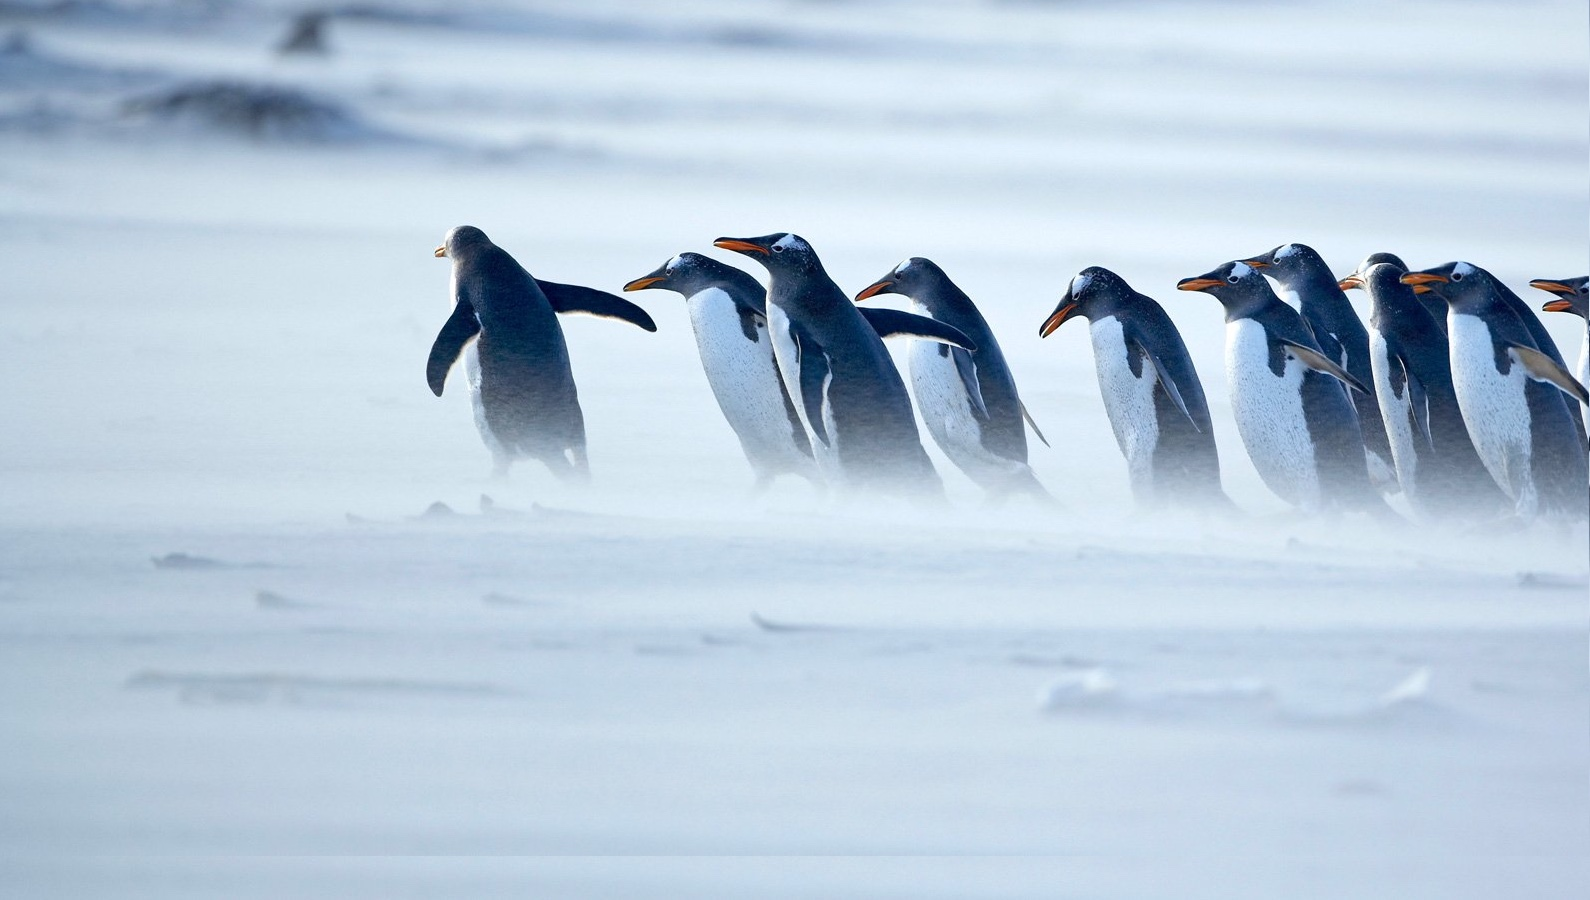
\includegraphics[height=\paperheight, width=\paperwidth]{pictures/leader.jpg}}
\begin{frame}
  \frametitle{Führung übernehmen}\framesubtitle{Proaktiv handeln}
  \note{ Wie kommt und bleibt man im Lead. (Driver Seat / Steuermann)
  \begin{itemize}
    \item In den Lead kommen: Gutes Offering - Beziehungen
    \item Im Lead Bleiben:
    \begin{itemize}
      \item Proaktiv handeln - Wir sind der Steuermann
      \item Beziehungen / Erwartungen
      \item Keine Ausreden
    \end{itemize}
  \end{itemize}
  STORY: Ralph: Erwartungen im Führungsteam nicht abgestimmt. Aber das ist ja nicht euer Problem. Ihr führt die Workshops durch.

  Ich: Unser Ziel ist es, dass unsere Kunden ihre Ziele erreichen.
  \begin{itemize}
    \item Workshop im Führungsteam
  \end{itemize}
  WICHTIG-WICHTIG - Überleitung Ziele - WICHTIG-WICHTIG
  }

\end{frame}

\usebackgroundtemplate{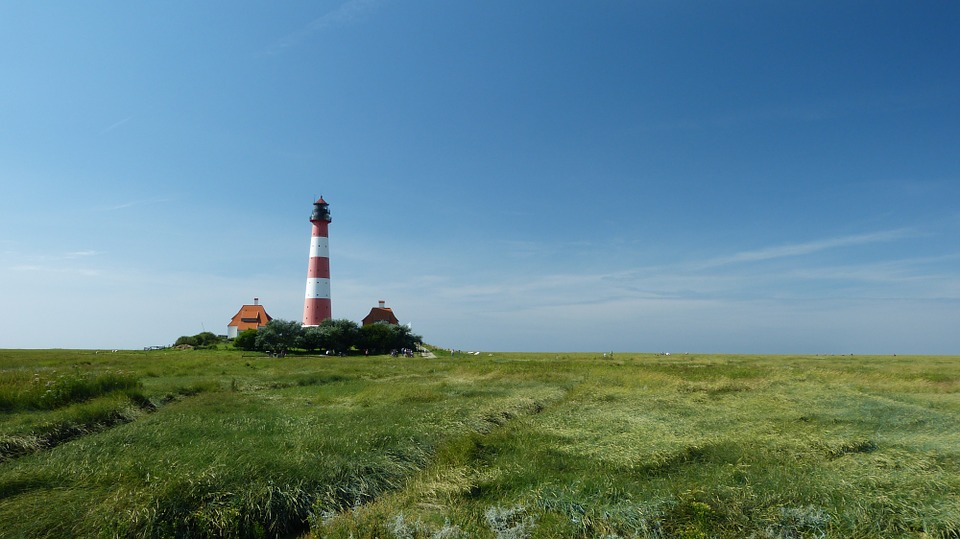
\includegraphics[height=\paperheight,width=\paperwidth]{pictures/leuchtturm.jpg}}
\begin{frame}
  \frametitle{Das Ziel immer vor Augen}\framesubtitle{Wissen was der Kunde wirklich will}
  \note{
  \begin{itemize}
    \item Erwartungen der Auftraggeber und der wichtigen Stakeholder erfüllen.
    \item Das Ziel steht nicht in der Offerte.
  \end{itemize}

  Story: In Workshops mit Führungsteams: Welche Fragen müssen am Schluss geklärt sein?
  \begin{itemize}
    \item Inwiefern ist die heutige IT Architektur/-strategie von der Einführung von DevOps betroffen?
    \item Welche Anpassungen sind für den Pilot am heutigen Helsana Release-Prozess erforderlich?
    \item Wo sind welche KPIs sinnvoll?
  \end{itemize}
  WICHTIG-WICHTIG - Überleitung Struktur - WICHTIG-WICHTIG
  \begin{itemize}
    \item Die Mannschaft zieht nur mit wenn sie den Plan kenn und vertraut
  \end{itemize}
  }
\end{frame}

\usebackgroundtemplate{
\includegraphics[height=\paperheight, width=\paperwidth]{pictures/wegweiser.jpg}}
\begin{frame}
  \frametitle{Vorgehensmodell}\framesubtitle{Struktur und ein Plan der aufgeht}
  \note{
  \begin{itemize}
    \item WHY ?
    \item WHEN ?
    \item Ein Plan muss wie eine Karte/Route sein (Beipiel Navi).
    \begin{itemize}
      \item Visualisiert
      \item Einprägsam
    \end{itemize}
  \end{itemize}
  Story: Vertrauen in den Plan war nicht klar. Reagiert.
  \begin{itemize}
    \item Vorgehensmodell $\rightarrow$ Framework
    \item Templates:
    \begin{itemize}
      \item Valuestream Map
      \item Visualisierung des myHelsana Development Streams
    \end{itemize}
  \end{itemize}


  WICHTIG-WICHTIG - Überleitung Expertise - WICHTIG-WICHTIG

  }
\end{frame}

\usebackgroundtemplate{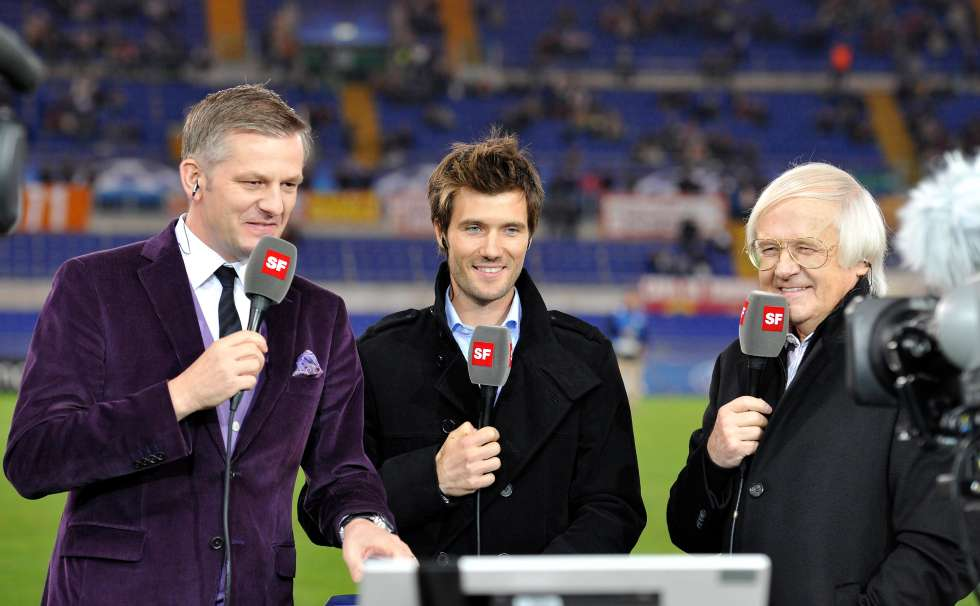
\includegraphics[height=\paperheight, width=\paperwidth]{pictures/experten.jpg}}
\begin{frame}
  \frametitle{Expertise}\framesubtitle{Glaubwürdigkeit durch Erfahrung}
  \note{
  \begin{itemize}
    \item Experten sind authentisch
    \item Experten haben Hands On Erfahrung
  \end{itemize}
  STORY: Bila Pascal Joos zum Thema Tooling in der Deployment Pipeline
  \begin{itemize}
    \item Technisch mitreden
    \item LiveDemo: Vagrant Ansible
    \item 4 Wochen später: Anfrage HARD Unterstützung
  \end{itemize}
  WICHTIG-WICHTIG - Überleitung Demo immer fit bleiben - WICHTIG-WICHTIG
  }
\end{frame}



\usebackgroundtemplate{
\includegraphics[height=\paperheight, width=\paperwidth]{pictures/engineering.jpg}}
\begin{frame}
\frametitle{Authentizität}\framesubtitle{Immer fit bleiben}
\note{2 min Infrastructure as Code Live Demo
\begin{itemize}
  \item Führung übernehmen.
  \item Ein gutes Ziel / Wirkung
  \item Vorgehensmodell oder Plan
  \item Expertise
\end{itemize}
}
\end{frame}

\usebackgroundtemplate{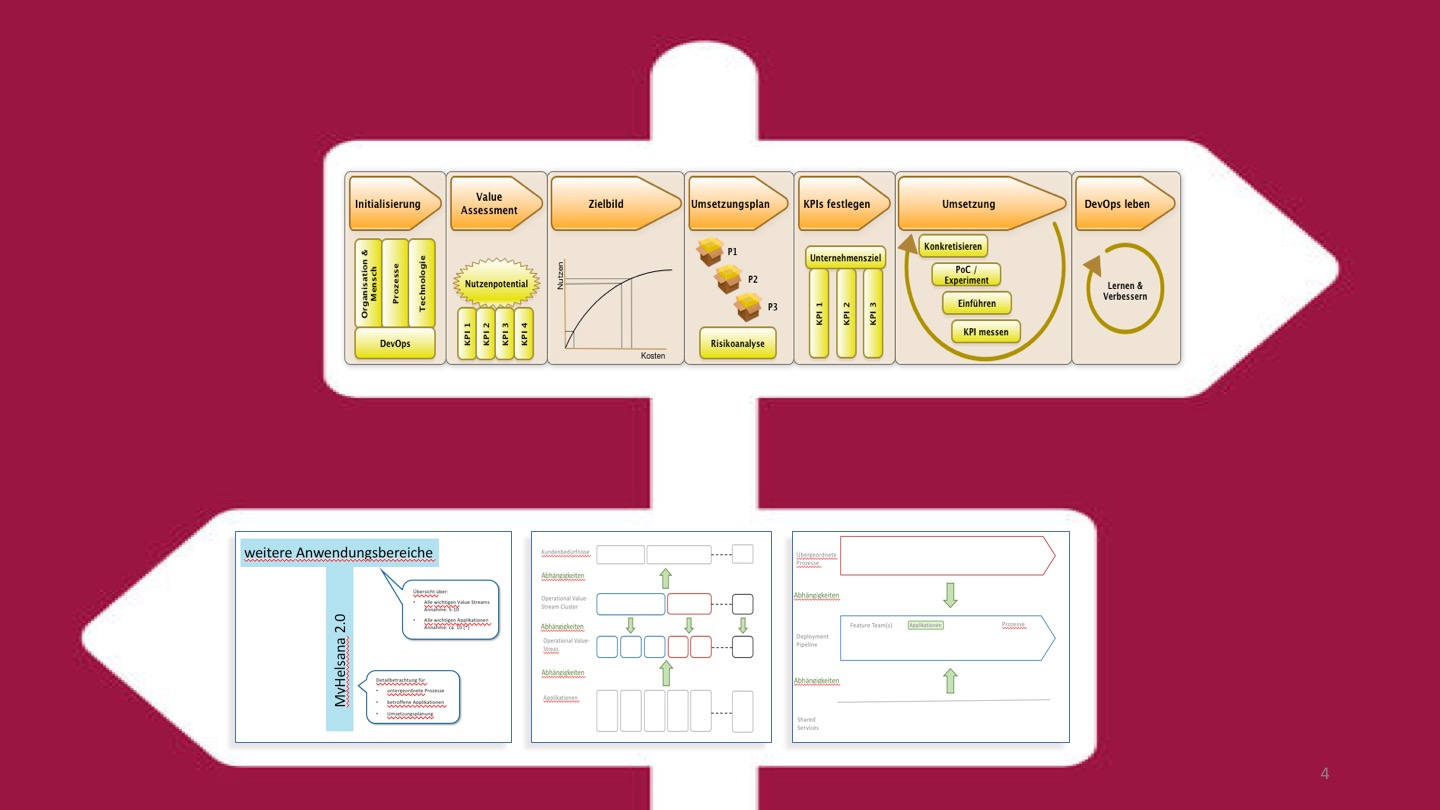
\includegraphics[height=\paperheight, width=\paperwidth]{pictures/framework.jpg}}
\begin{frame}
\note{Framework}
\end{frame}

\usebackgroundtemplate{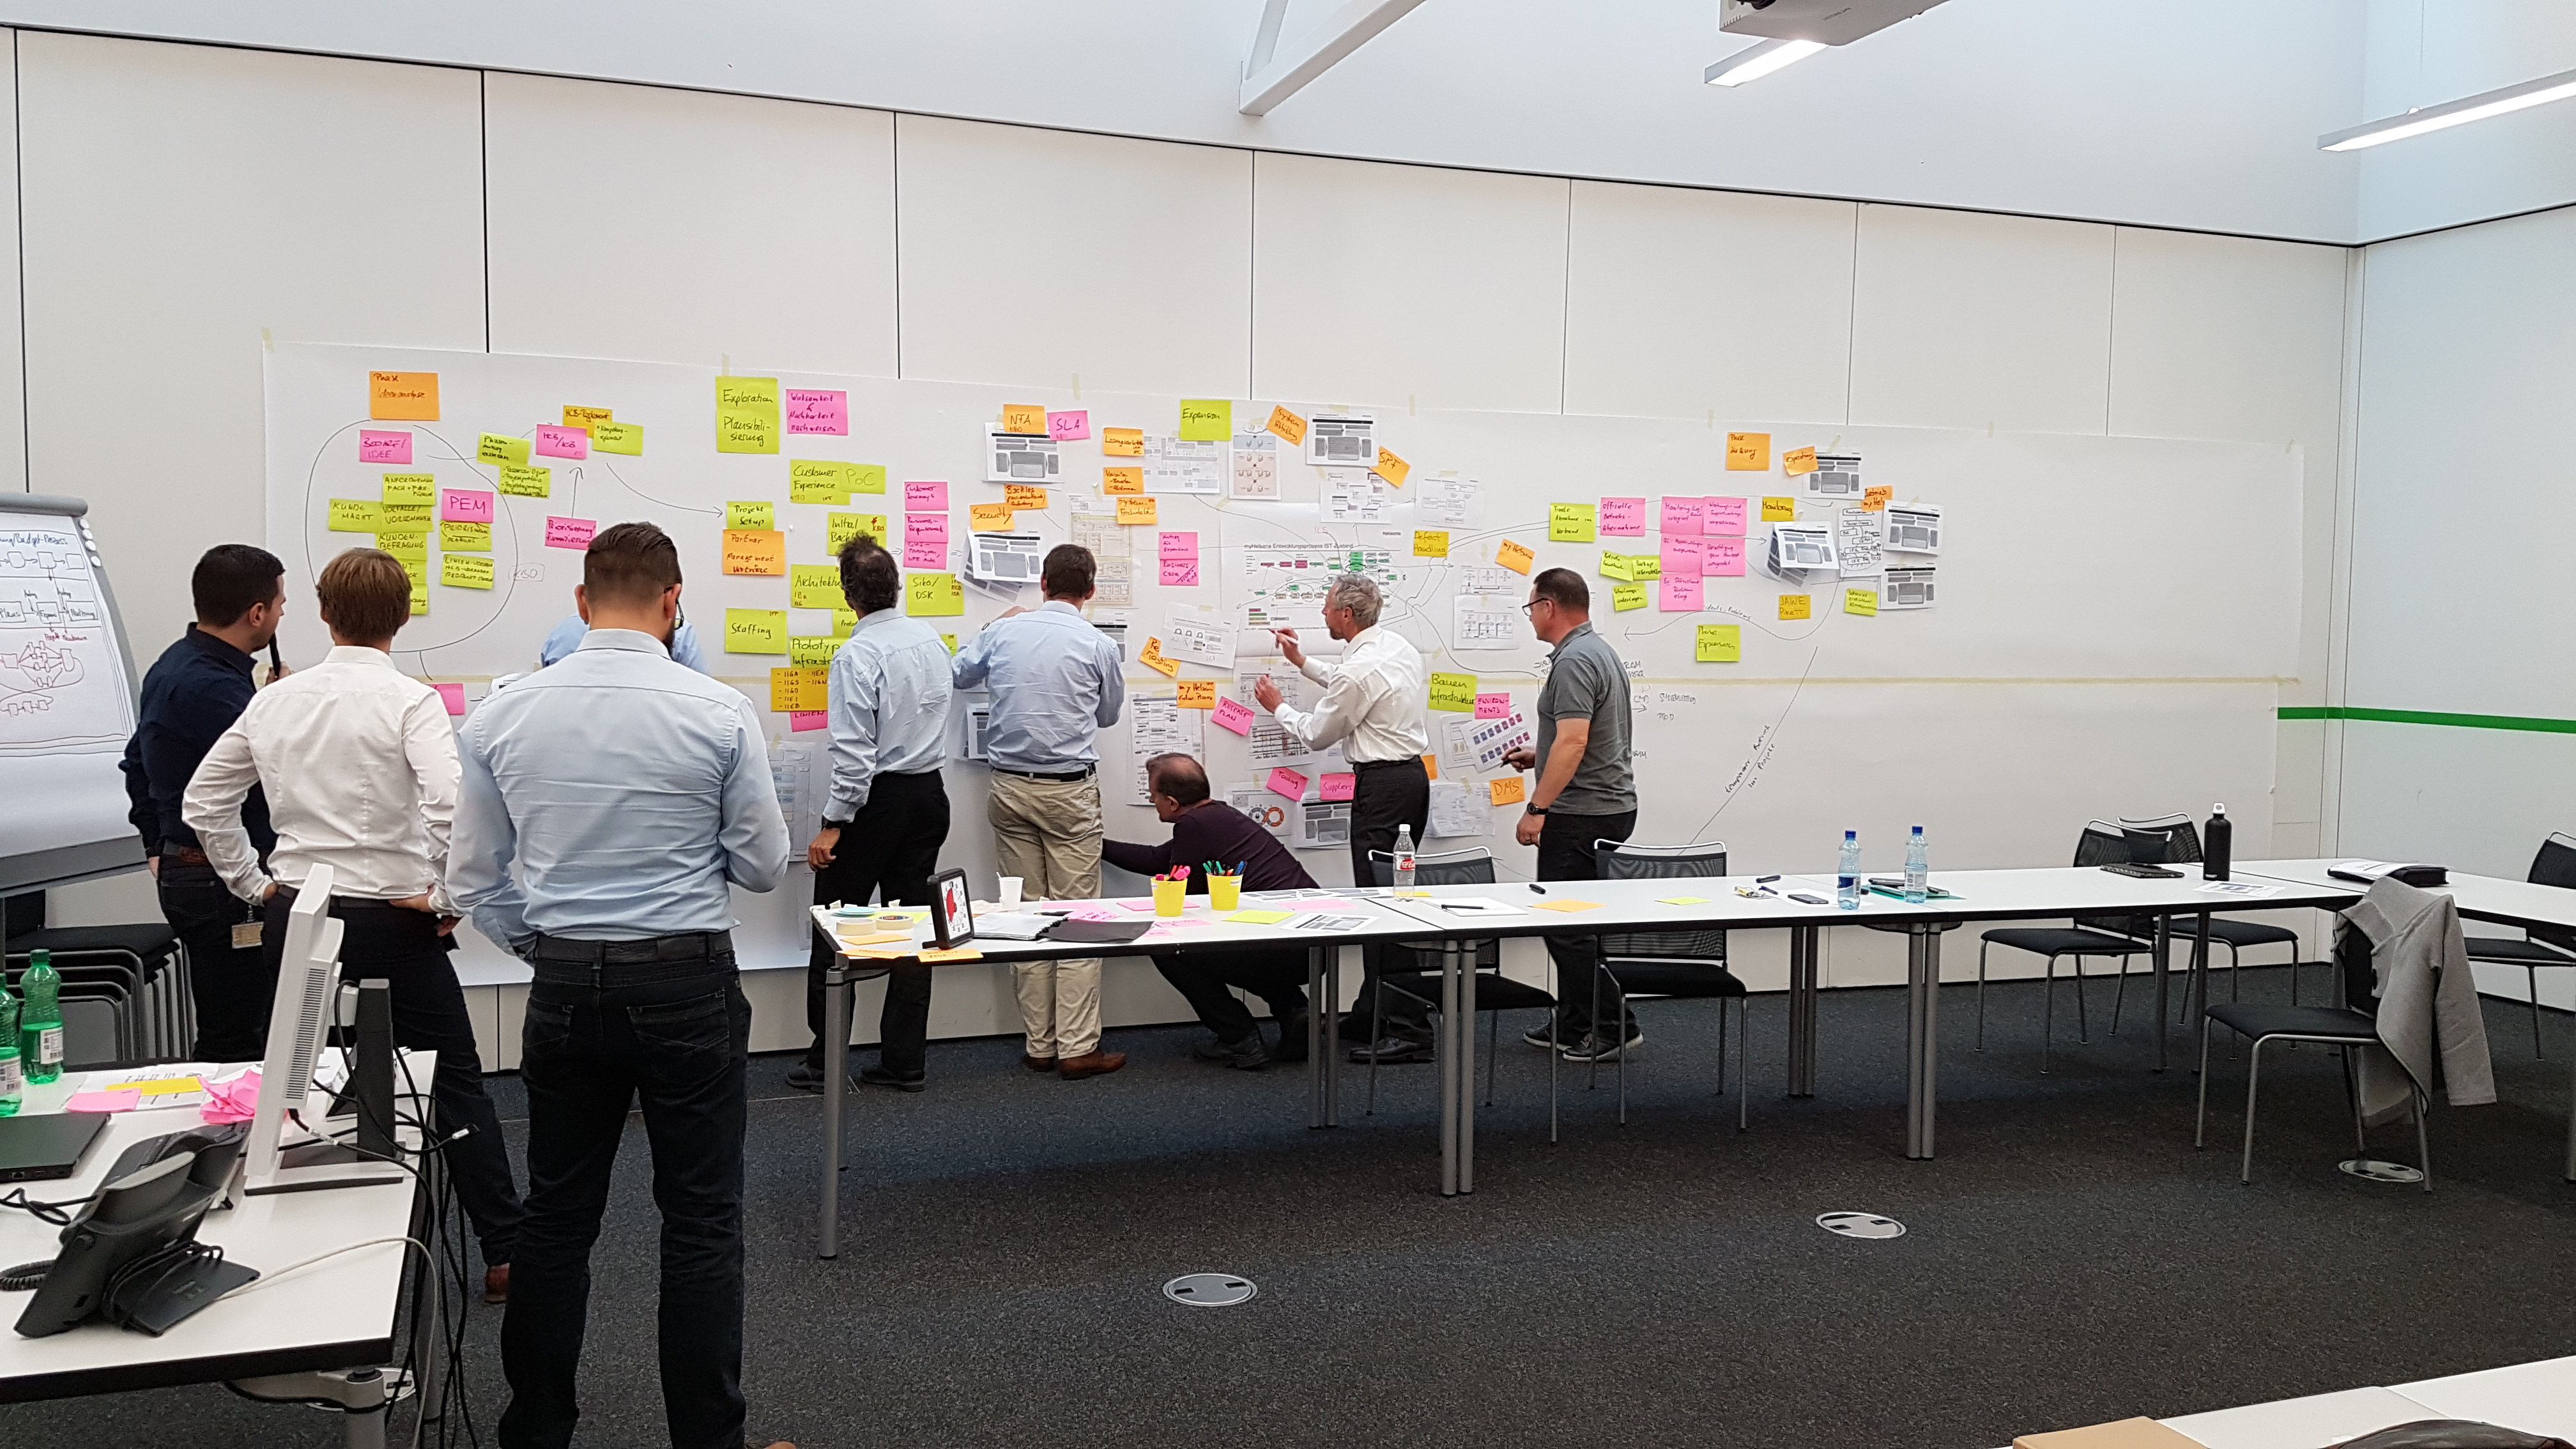
\includegraphics[height=\paperheight, width=\paperwidth]{pictures/ausgangslage.jpg}}
\begin{frame}
\note{Ausgangslage}
\end{frame}

\usebackgroundtemplate{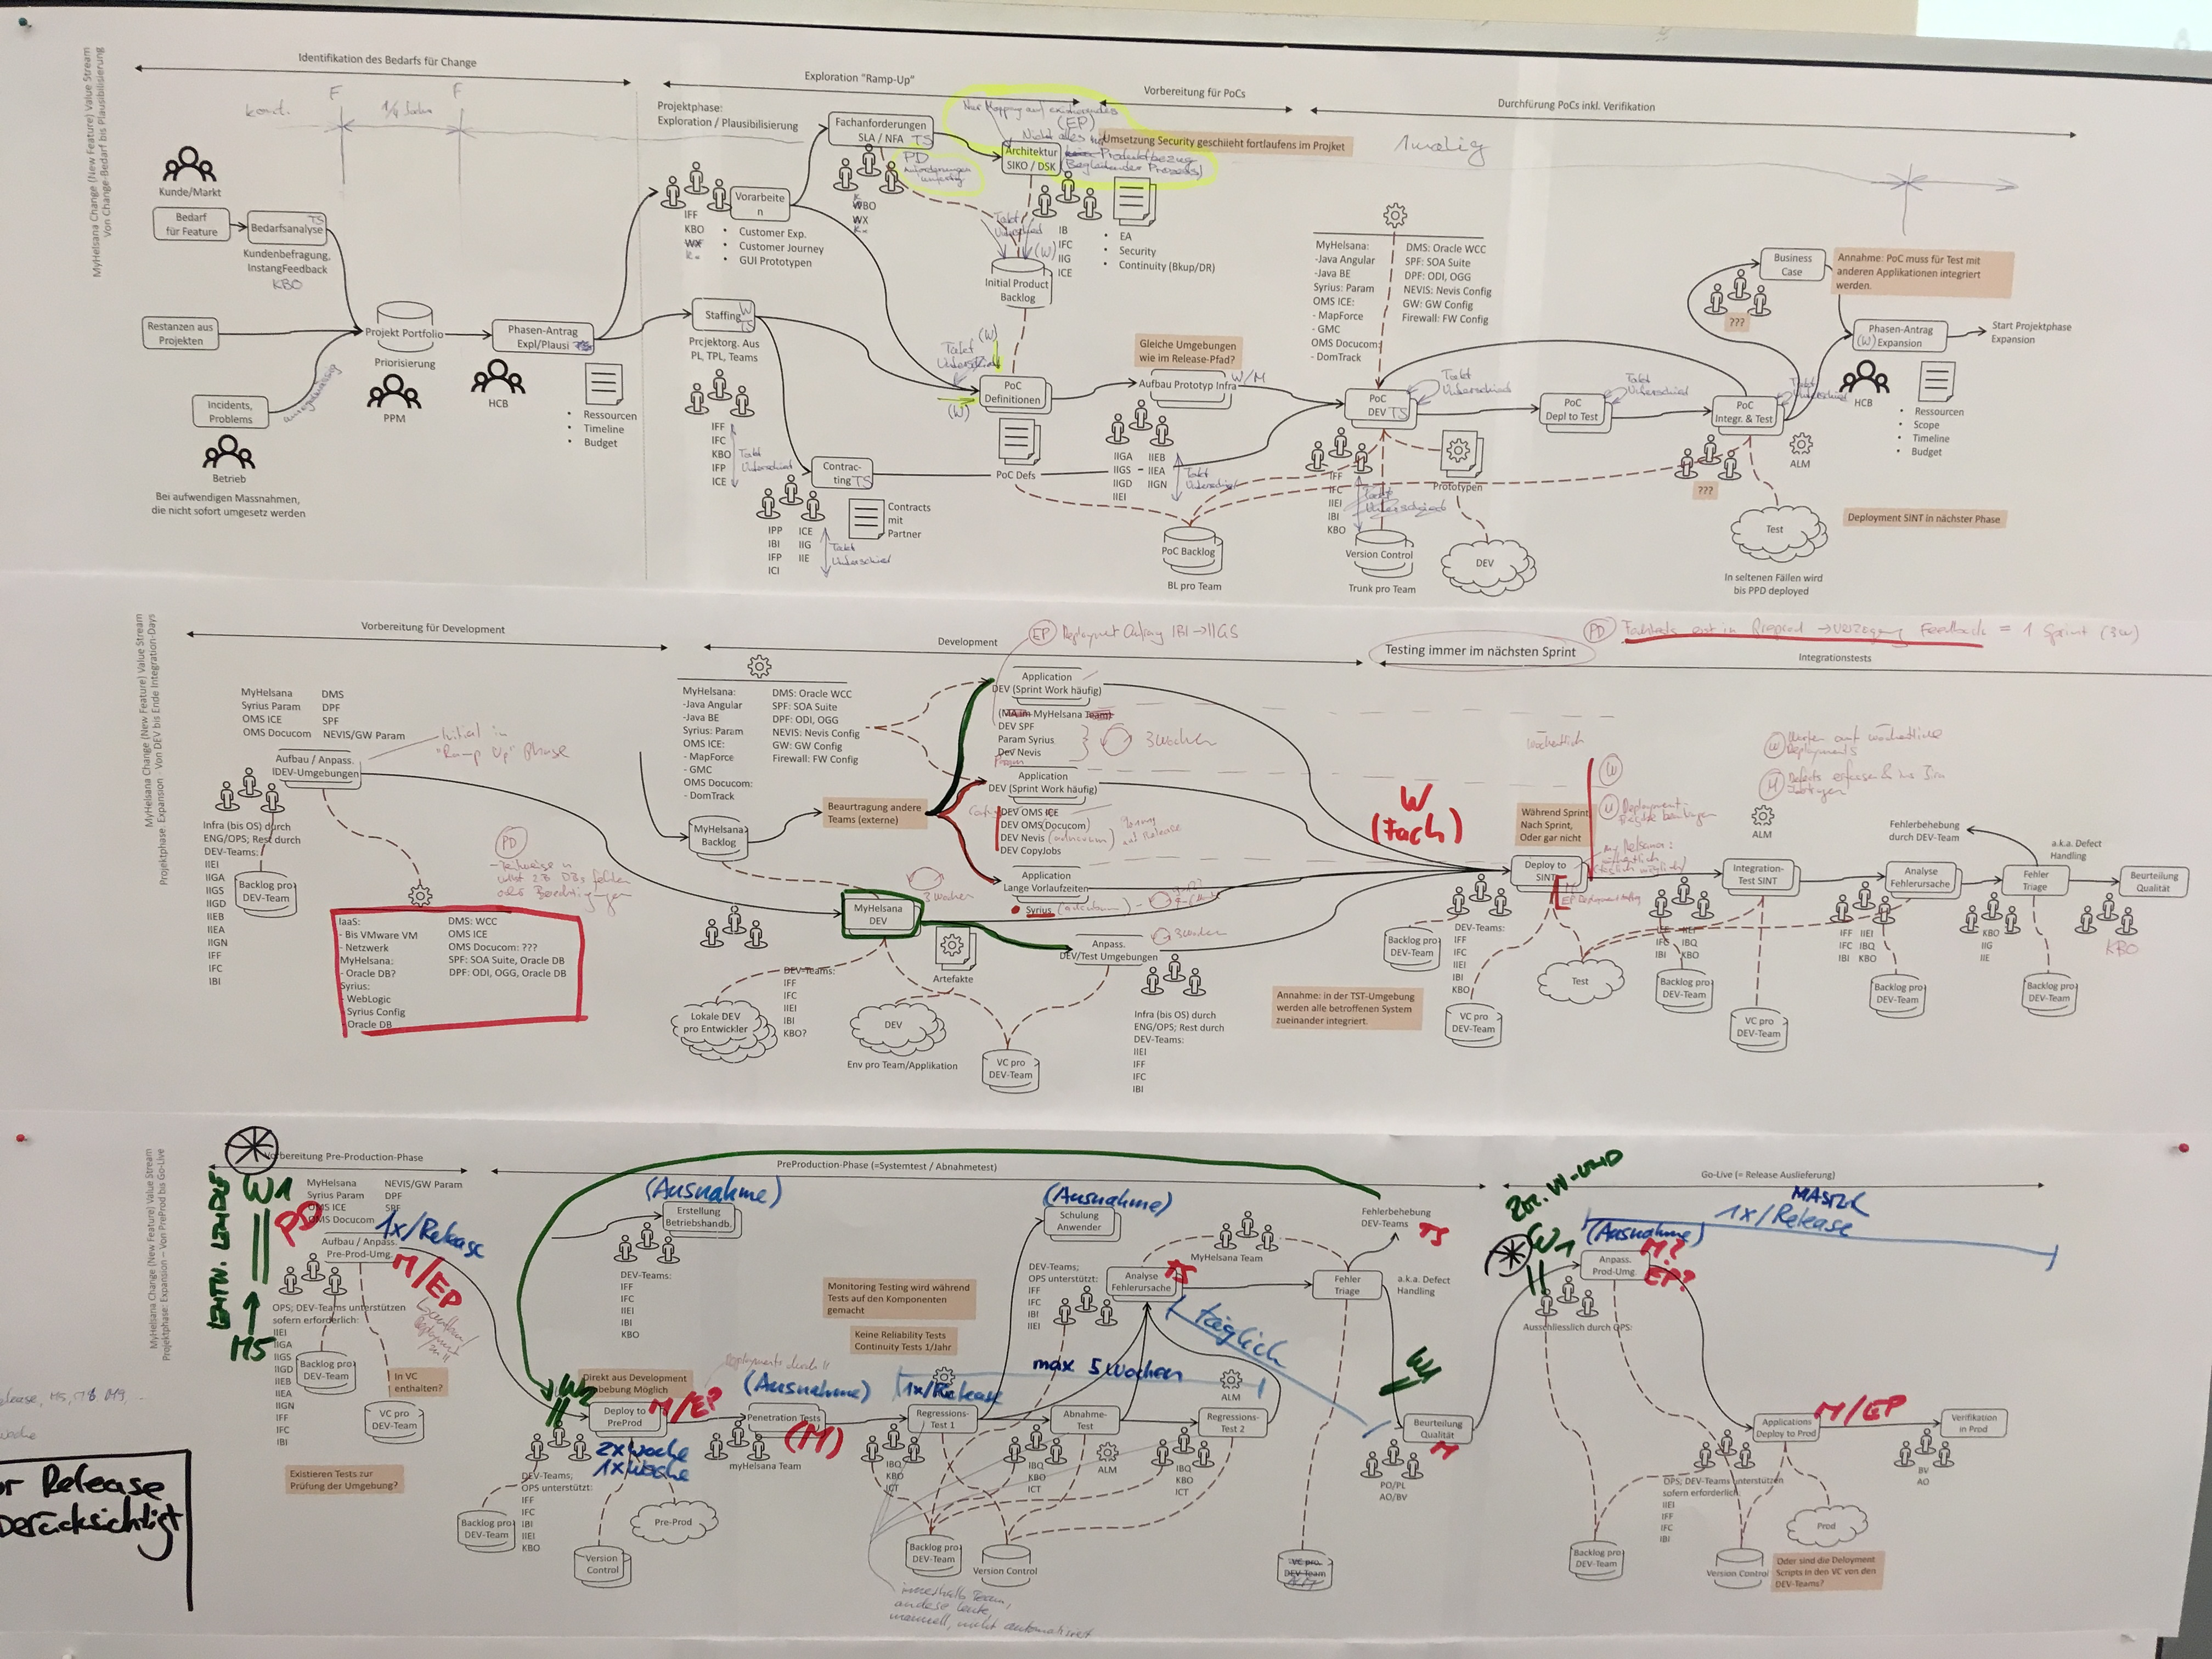
\includegraphics[width=\paperwidth]{pictures/vsm.jpg}}
\begin{frame}
\note{Value Stream Mapping myHeldana}
\end{frame}

\usebackgroundtemplate{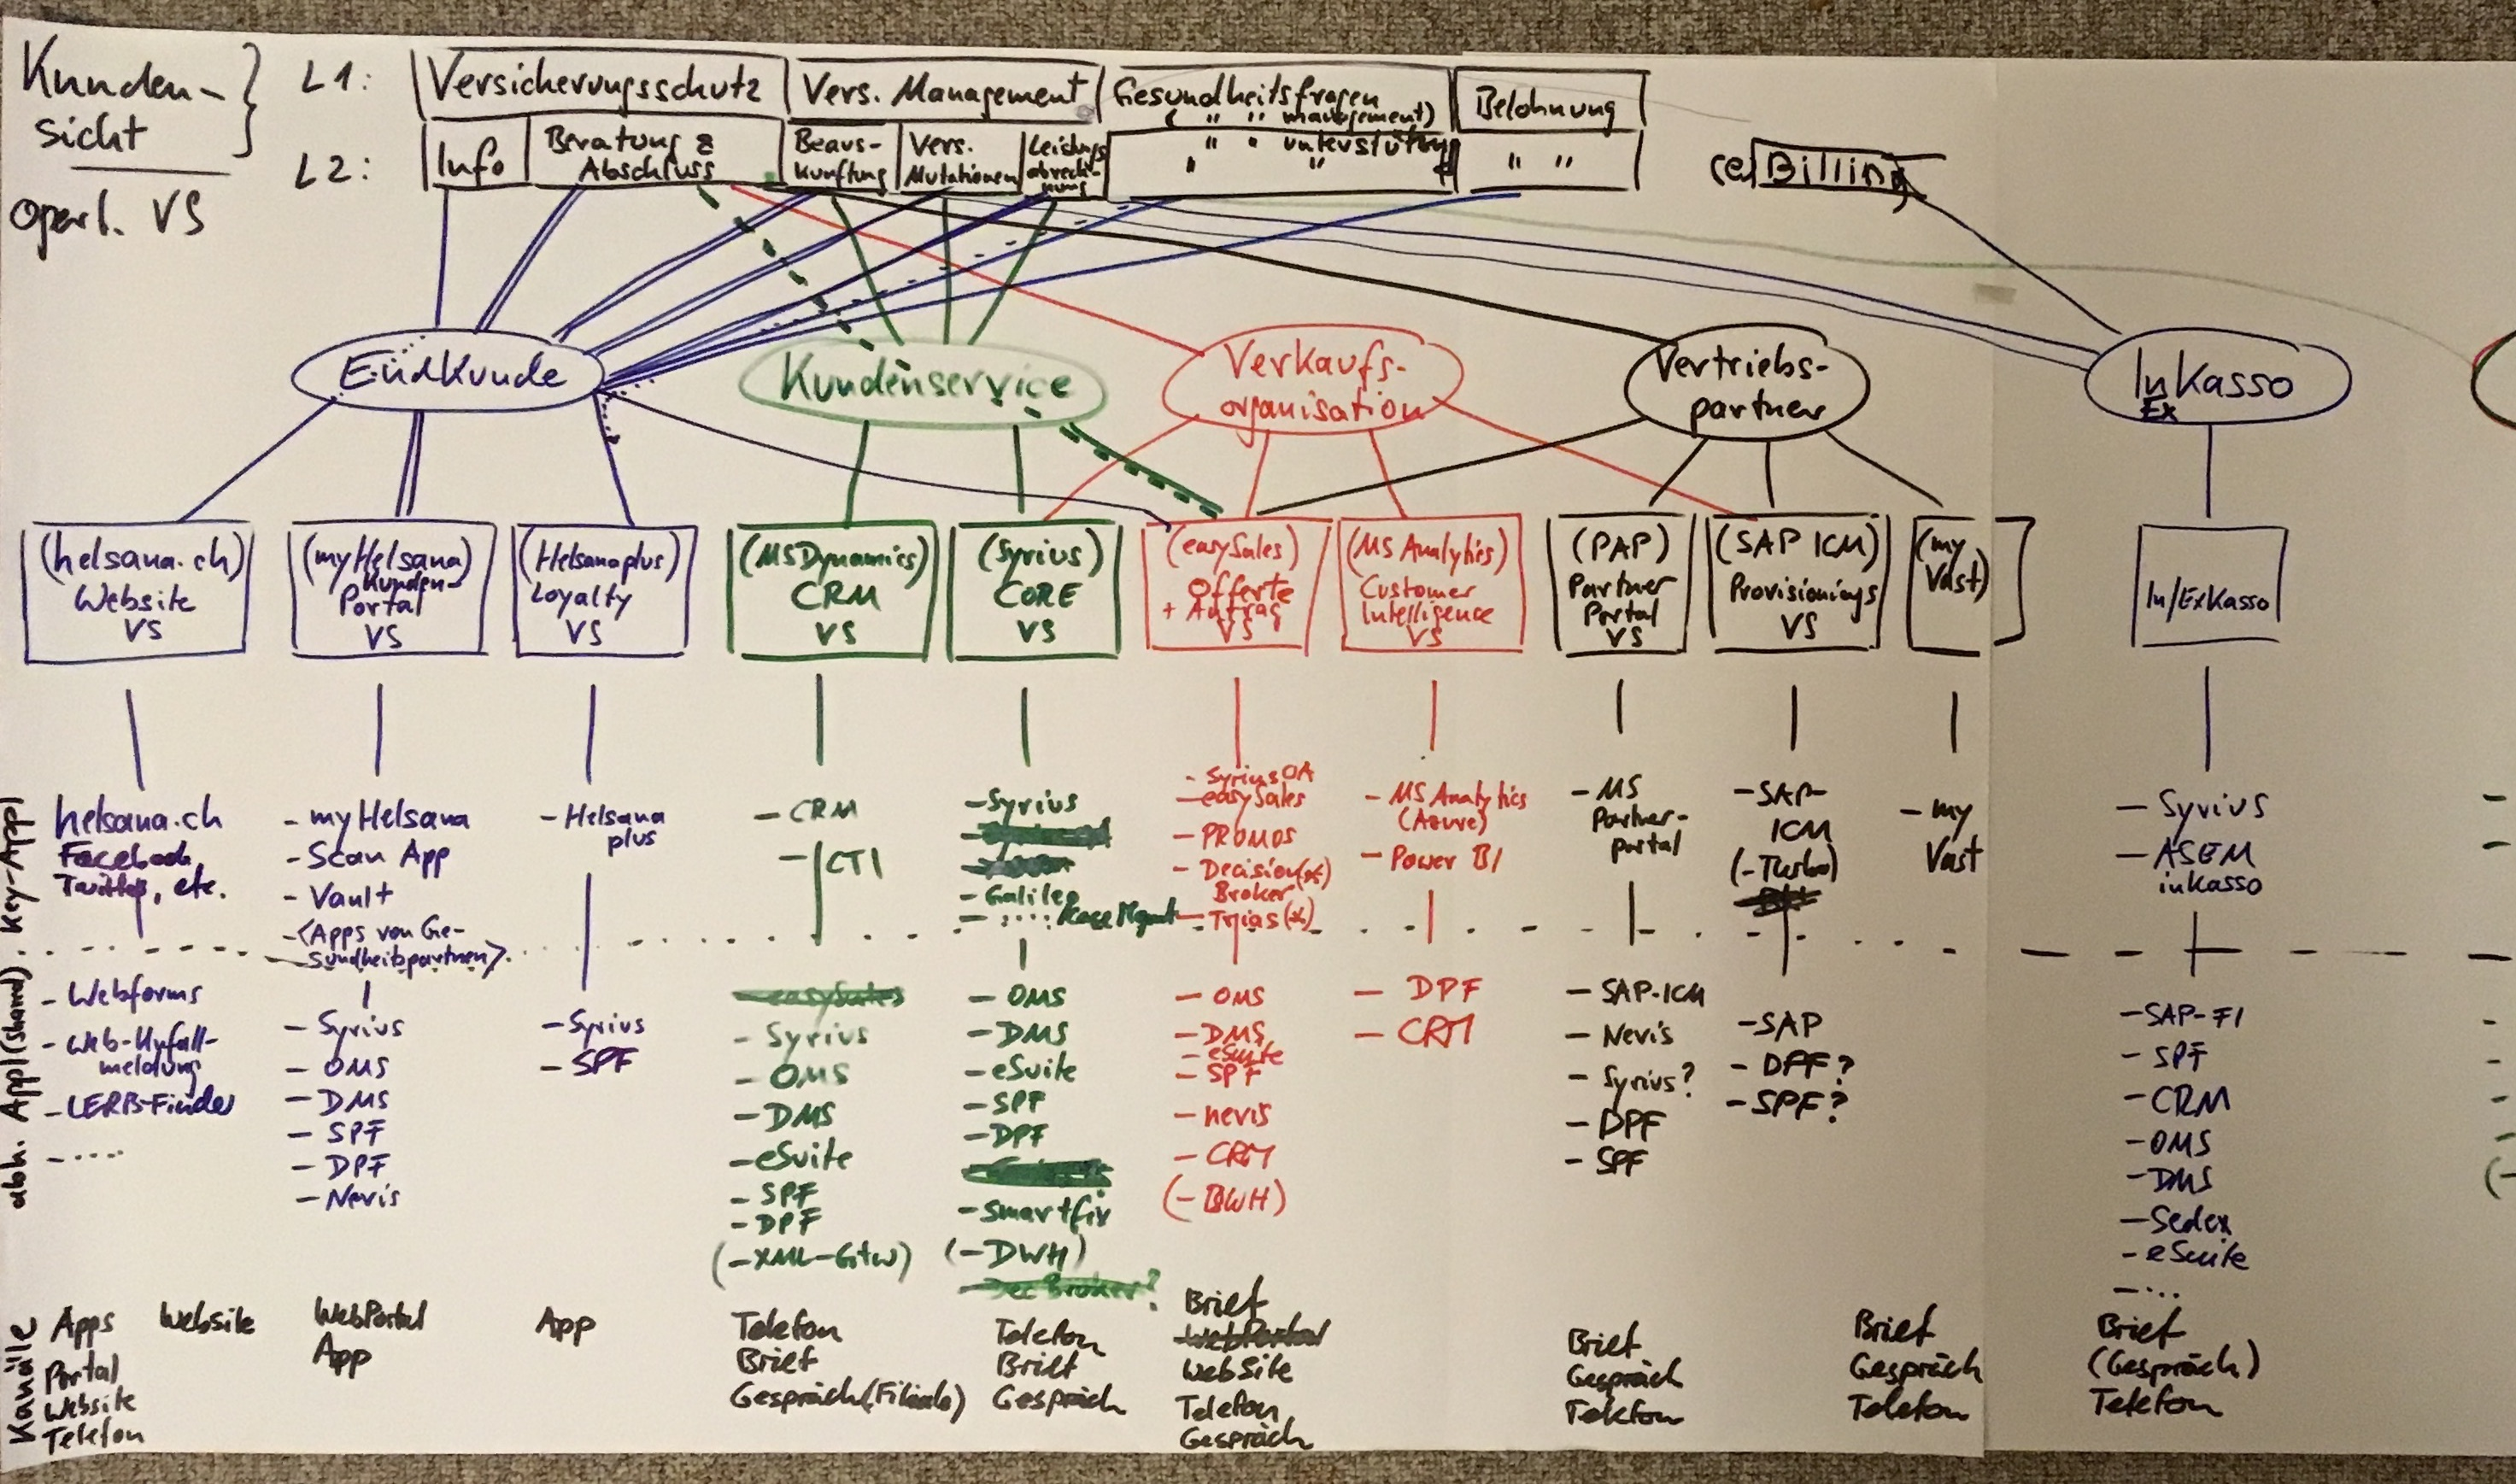
\includegraphics[height=\paperheight, width=\paperwidth]{pictures/vs_uebersicht.jpg}}
\begin{frame}
\note{Übersicht über alle Helsana Value Streams}
\end{frame}

\usebackgroundtemplate{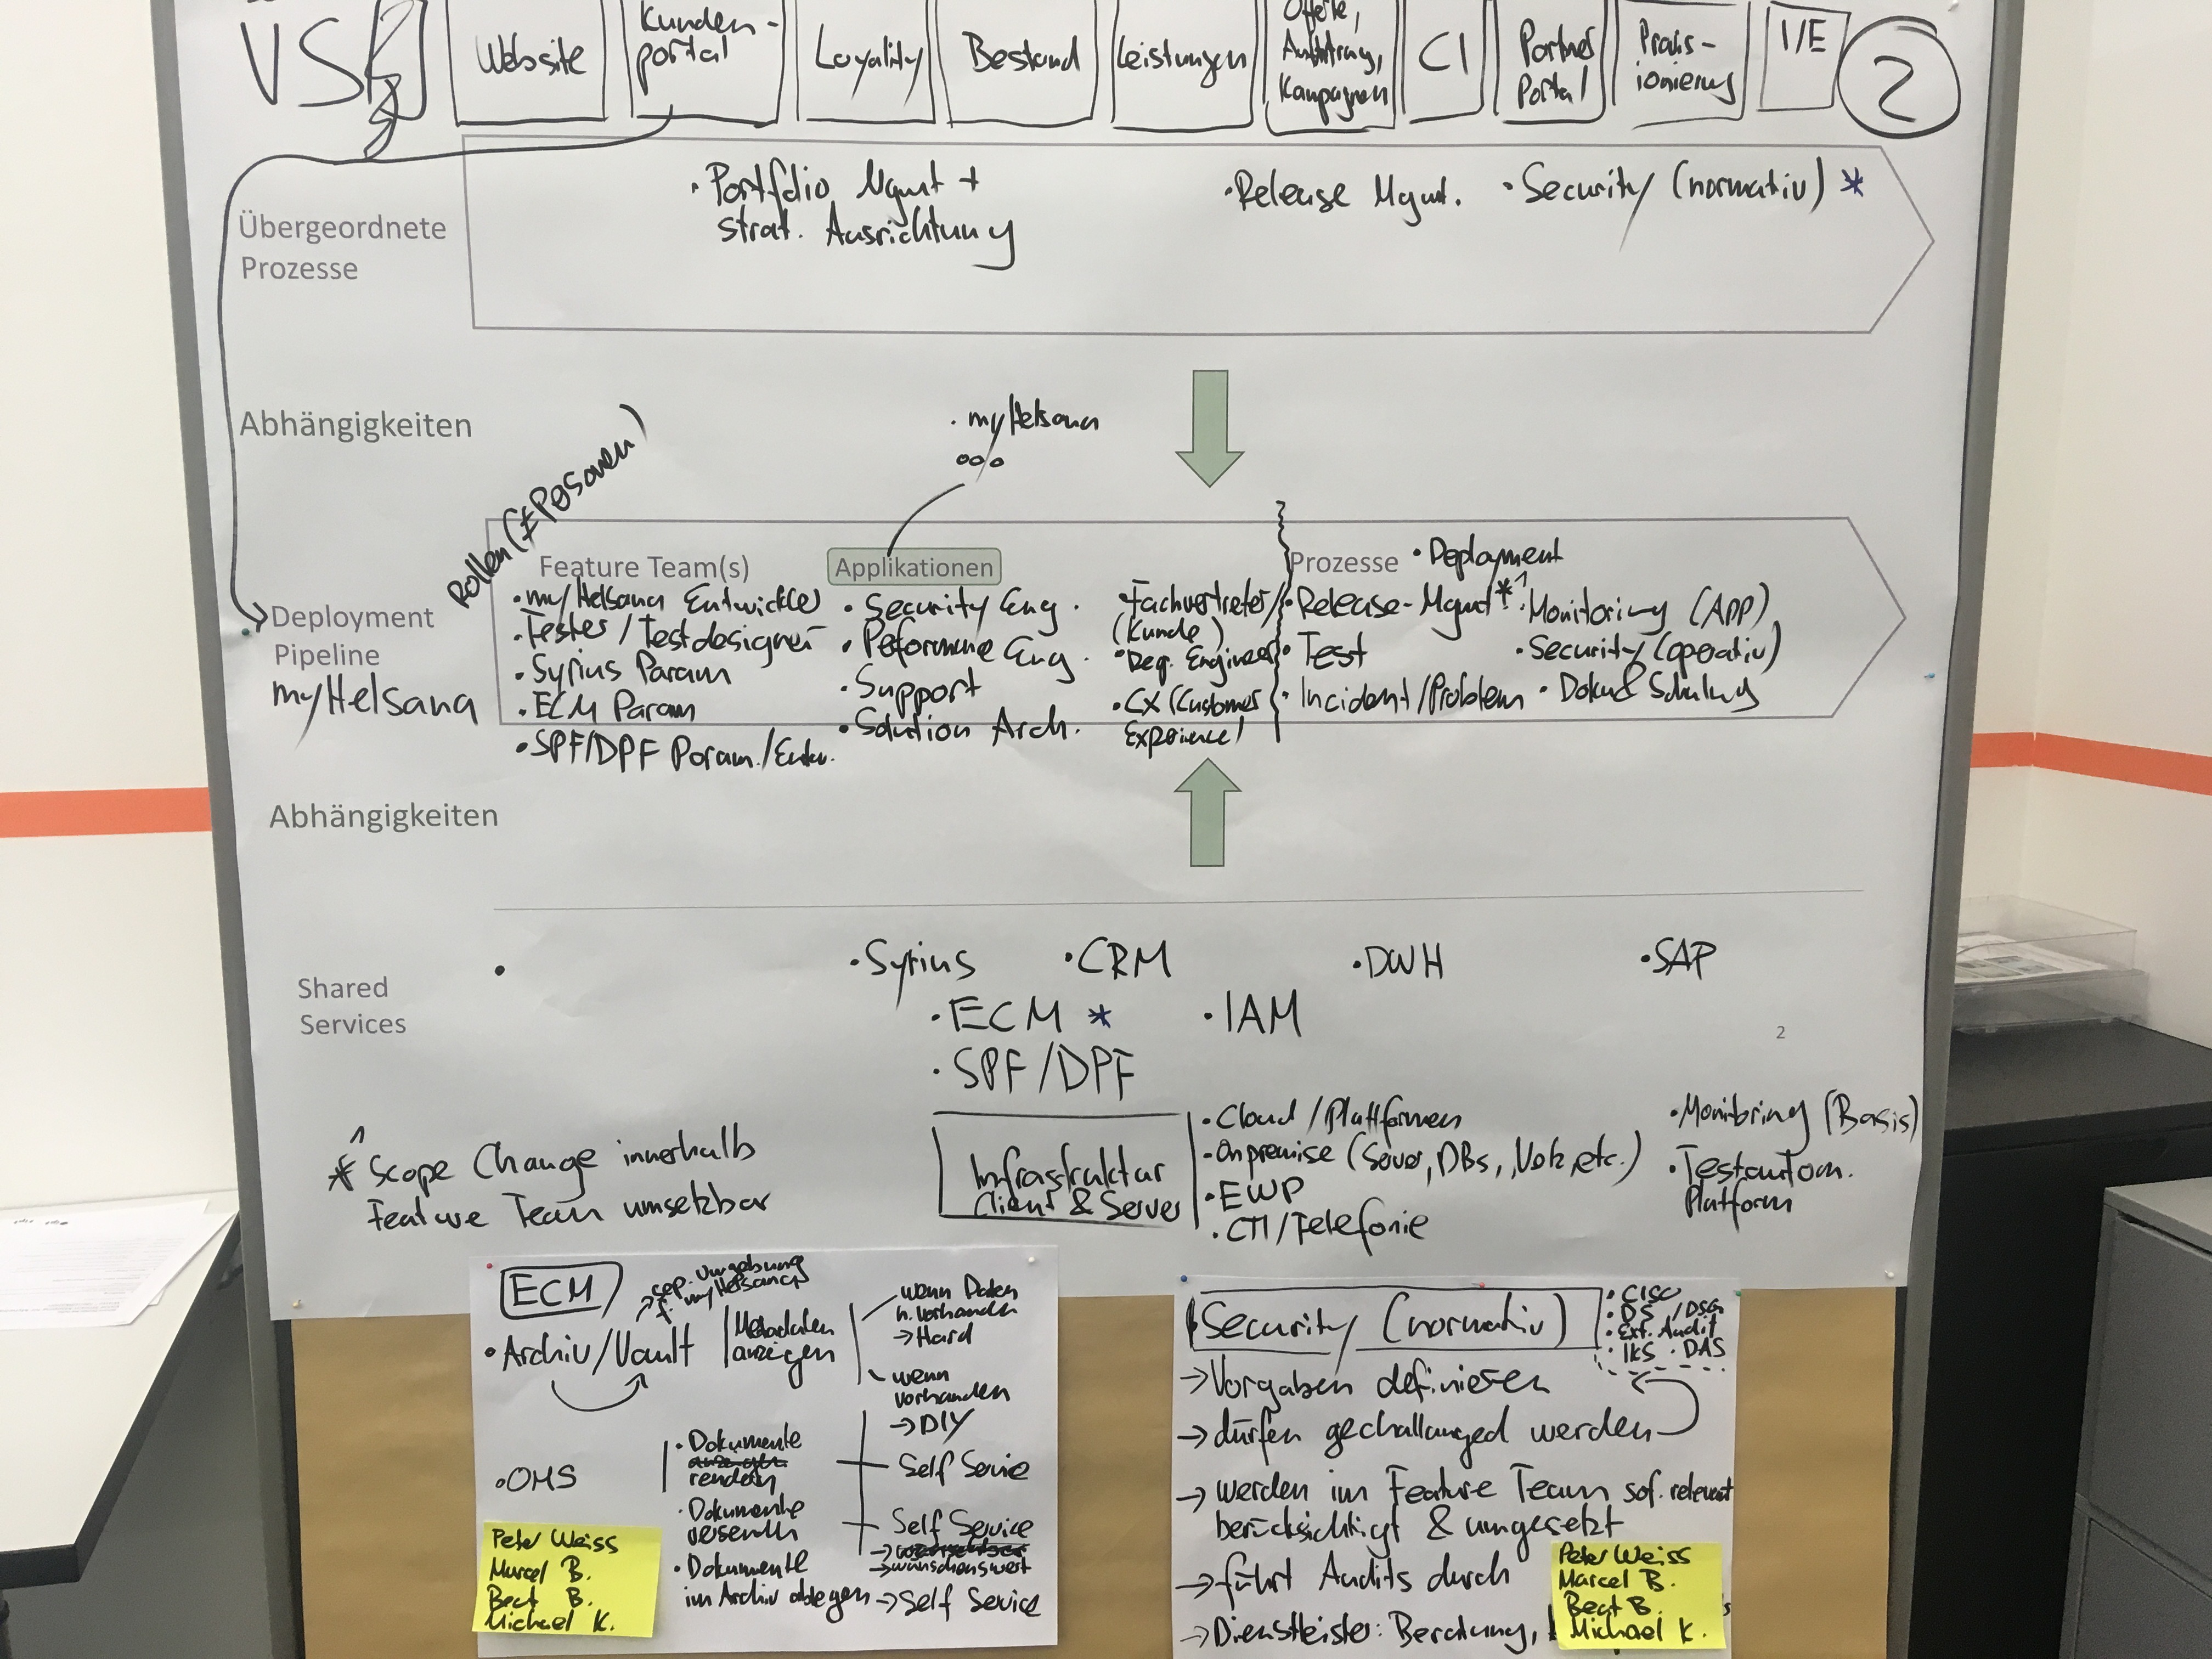
\includegraphics[height=\paperheight, width=\paperwidth]{pictures/zielbildIteration2.jpg}}
\begin{frame}
\note{Verfollständigung des Zielbild}
\end{frame}


\usebackgroundtemplate{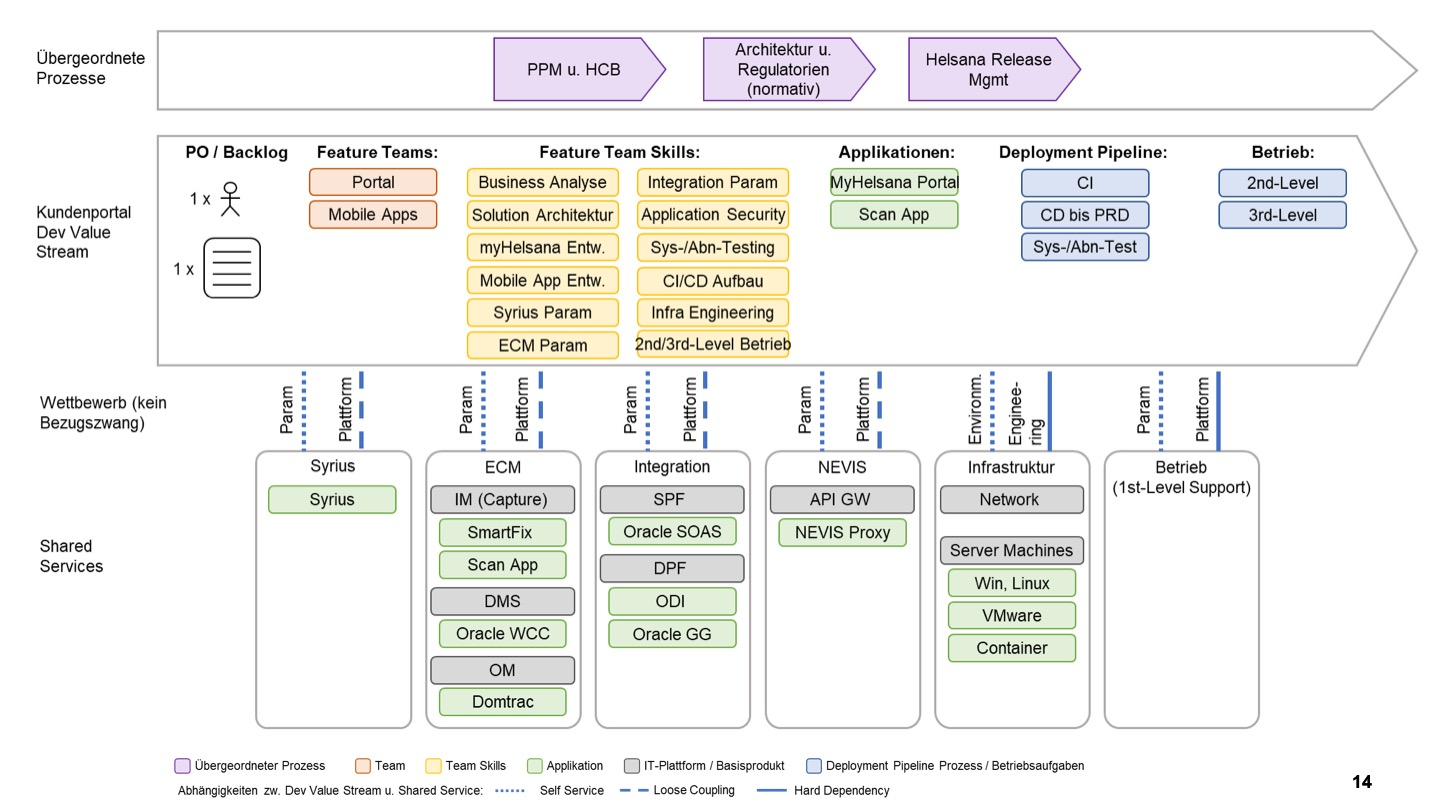
\includegraphics[height=\paperheight, width=\paperwidth]{pictures/zielbildFinal.jpg}}
\begin{frame}
\note{Finale Version des Helsana BizDevOps Zielbild (Graphik)}
\end{frame}

\usebackgroundtemplate{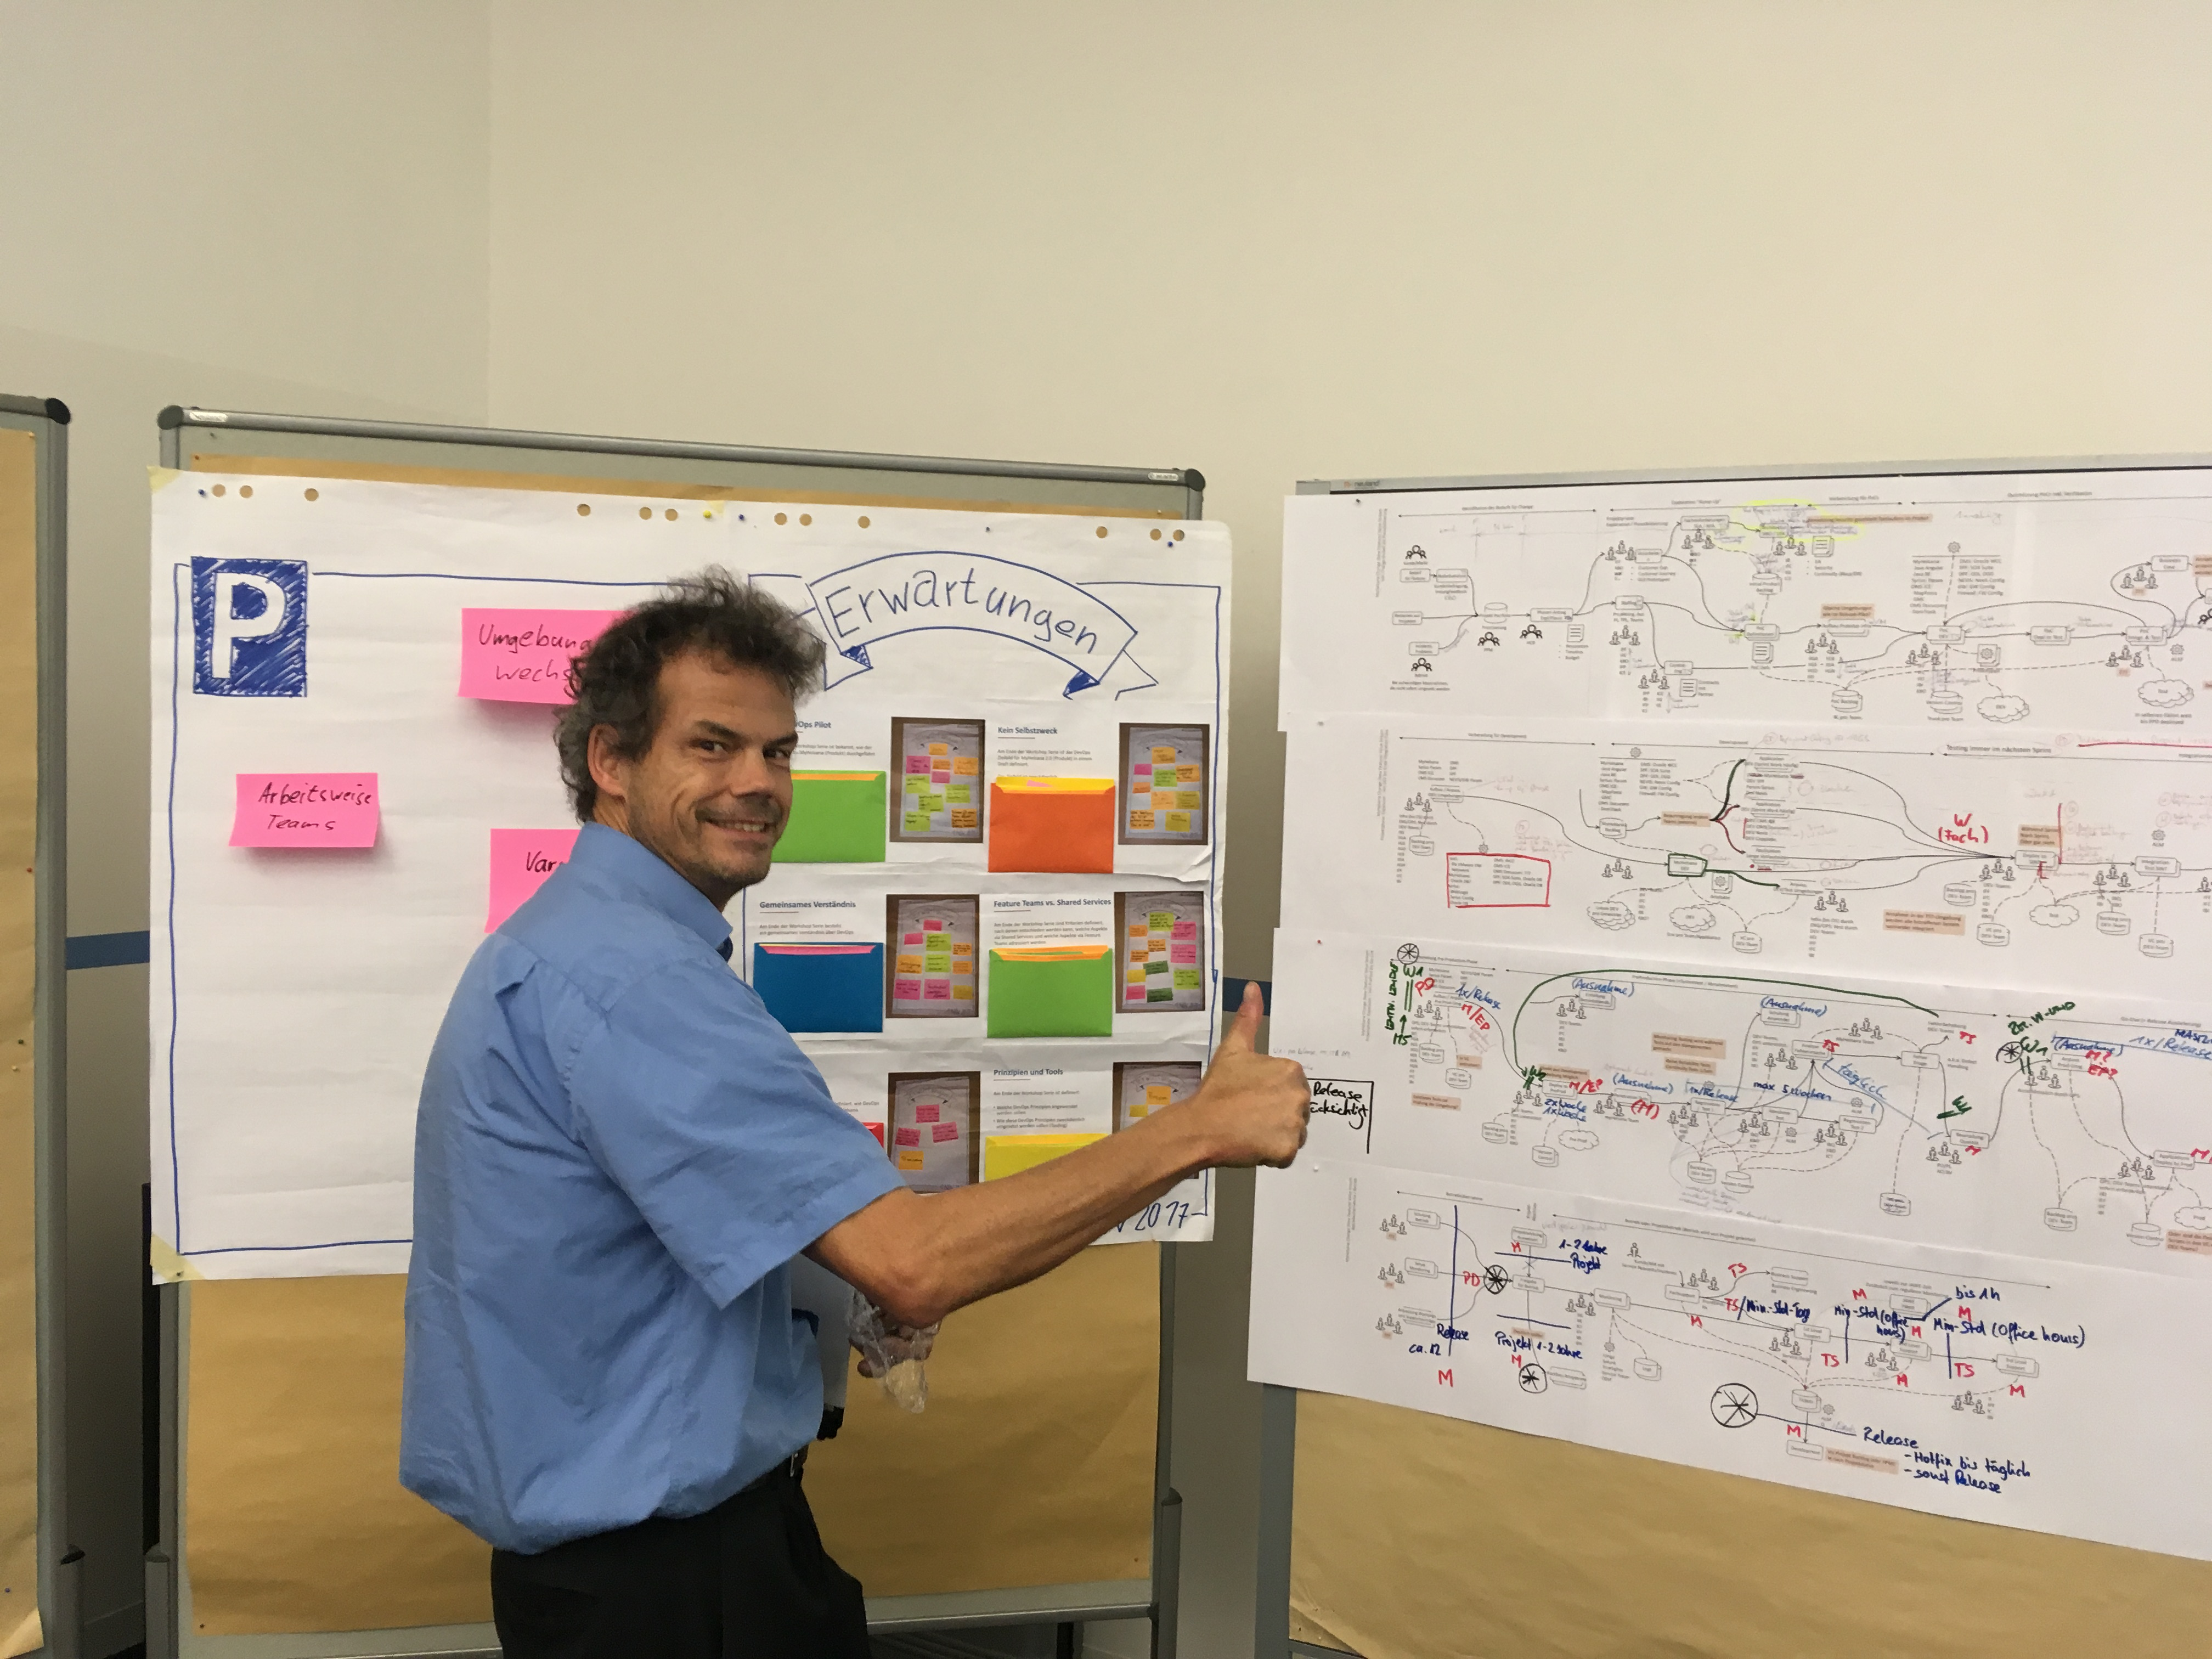
\includegraphics[height=\paperheight, width=\paperwidth]{pictures/samuel_hat_spass.png}}
\begin{frame}
  \note{Es geht weiter / Business Value DevOps
  \begin{itemize}
    \item Führung übernehmen.
    \item Ein gutes Ziel / Wirkung
    \item Vorgehensmodell oder Plan
    \item Expertise
  \end{itemize}
  }
\end{frame}

\end{document}
